\documentclass[12pt]{article}

% Packages
\usepackage[a4paper, margin=1in]{geometry}
\usepackage{amsmath}
\usepackage{graphicx}
\usepackage{caption}
\usepackage{listings}
\usepackage{xcolor}
\usepackage{titlesec}
\usepackage{fancyhdr}
\usepackage{hyperref}
\usepackage{placeins} % <-- Added to control float positions

% Header and Footer
\pagestyle{fancy}
\fancyhf{}
\rhead{Experiment 4}
\lhead{Distribution Functions in Python}
\rfoot{\thepage}

% Section formatting
\titleformat{\section}{\large\bfseries}{\thesection}{1em}{}
\titleformat{\subsection}{\normalsize\bfseries}{\thesubsection}{1em}{}

% Code Styling
\lstset{
  basicstyle=\ttfamily\small,
  keywordstyle=\color{blue},
  stringstyle=\color{green!60!black},
  commentstyle=\color{gray}\itshape,
  breaklines=true,
  frame=single,
  numbers=left,
  numberstyle=\tiny,
  numbersep=5pt,
  backgroundcolor=\color{gray!10},
  tabsize=2
}

\begin{document}

\begin{center}
    \Large \textbf{Experiment 4: Distribution Functions in Python} \\
    \normalsize \textbf{Using Uniform, Normal, and Exponential Distributions}
\end{center}

\vspace{1em}

\section*{Objective}
To generate and visualize random values from three different statistical distributions using Python:
\begin{itemize}
    \item Uniform Distribution
    \item Normal Distribution
    \item Exponential Distribution
\end{itemize}

\section*{Tools Used}
\begin{itemize}
    \item Python 3
    \item NumPy
    \item Matplotlib
    \item SciPy (scipy.stats)
\end{itemize}

\section*{Theory}
\subsection*{1. Uniform Distribution}
A uniform distribution has constant probability. Each value within a specific interval is equally likely to occur. In \texttt{scipy.stats.uniform}, the parameters are:
\begin{itemize}
    \item \texttt{loc}: The start of the interval.
    \item \texttt{scale}: The width of the interval.
\end{itemize}

\subsection*{2. Normal Distribution}
Also known as the Gaussian distribution. It is symmetric around the mean. The parameters are:
\begin{itemize}
    \item \texttt{loc}: The mean of the distribution.
    \item \texttt{scale}: The standard deviation.
\end{itemize}

\subsection*{3. Exponential Distribution}
Models the time between events in a Poisson process. The parameter is:
\begin{itemize}
    \item \texttt{scale}: Equal to \( \frac{1}{\lambda} \) where \( \lambda \) is the rate.
\end{itemize}

\section*{Python Code}

\subsection*{Import Libraries and Set Seed}
\begin{lstlisting}[language=Python]
import numpy as np
import matplotlib.pyplot as plt
from scipy.stats import uniform, norm, expon

# Set seed for reproducibility
np.random.seed(42)
\end{lstlisting}

\subsection*{1. Uniform Distribution}
\begin{lstlisting}[language=Python]
# Uniform Distribution: loc = start, scale = width
uniform_data = uniform.rvs(loc=0, scale=10, size=1000)

plt.figure(figsize=(10, 4))
plt.hist(uniform_data, bins=30, density=True, alpha=0.6, 
         color='skyblue', edgecolor='black')
plt.title('Uniform Distribution (loc=0, scale=10)')
plt.xlabel('Value')
plt.ylabel('Density')
plt.grid(True)
plt.savefig('uniform.png')
plt.show()
\end{lstlisting}

\subsection*{2. Normal Distribution}
\begin{lstlisting}[language=Python]
# Normal Distribution: loc = mean, scale = std deviation
normal_data = norm.rvs(loc=0, scale=1, size=1000)

plt.figure(figsize=(10, 4))
plt.hist(normal_data, bins=30, density=True, alpha=0.6, 
         color='lightgreen', edgecolor='black')
plt.title('Normal Distribution (mean=0, std=1)')
plt.xlabel('Value')
plt.ylabel('Density')
plt.grid(True)
plt.savefig('normal.png')
plt.show()
\end{lstlisting}

\subsection*{3. Exponential Distribution}
\begin{lstlisting}[language=Python]
# Exponential Distribution: scale = 1/lambda
exponential_data = expon.rvs(scale=1.0, size=1000)

plt.figure(figsize=(10, 4))
plt.hist(exponential_data, bins=30, density=True, alpha=0.6, 
         color='salmon', edgecolor='black')
plt.title('Exponential Distribution (scale=1.0)')
plt.xlabel('Value')
plt.ylabel('Density')
plt.grid(True)
plt.savefig('exponential.png')
plt.show()
\end{lstlisting}

\section*{Output Plots}

\begin{figure}[h!]
    \centering
    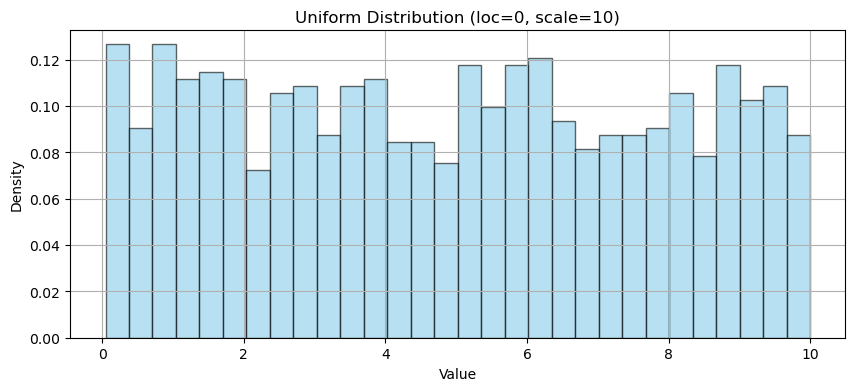
\includegraphics[width=0.8\linewidth]{unifrom distribution.png}
    \caption{Uniform Distribution (loc=0, scale=10)}
\end{figure}

\begin{figure}[h!]
    \centering
    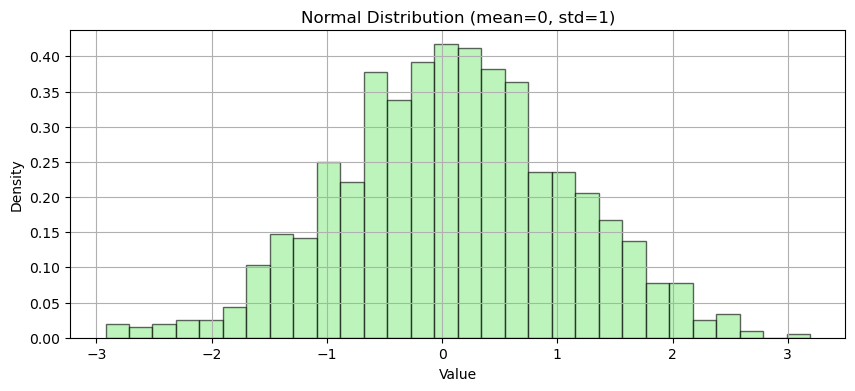
\includegraphics[width=0.8\linewidth]{Normal distribution.png}
    \caption{Normal Distribution (mean=0, std=1)}
\end{figure}

\begin{figure}[h!]
    \centering
    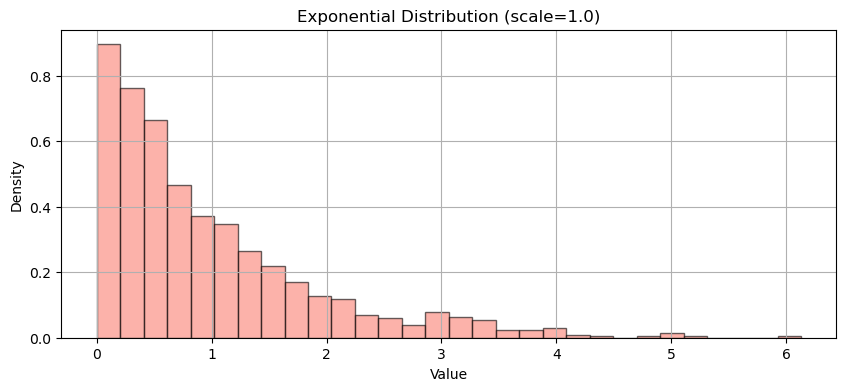
\includegraphics[width=0.8\linewidth]{exponential distribution.png}
    \caption{Exponential Distribution (scale=1.0)}
\end{figure}

\FloatBarrier  % <-- This keeps figures before conclusion

\section*{Conclusion}
This experiment successfully demonstrated how to generate and visualize data from uniform, normal, and exponential distributions using Python. The \texttt{scipy.stats} library offers a convenient interface to handle random variable generation and the associated parameters like \texttt{loc} and \texttt{scale}.

\end{document}
